\documentclass{article}

\usepackage{fancyhdr}
\usepackage{extramarks}
\usepackage{amsmath}
\usepackage{amsthm}
\usepackage{amsfonts}
\usepackage{tikz}
\usepackage[plain]{algorithm}
\usepackage{algpseudocode}
\usepackage{enumitem}
\usepackage{pgfplots}
\usepackage{subcaption}

\usetikzlibrary{automata,positioning}

% Basic document settings
\topmargin=-0.45in
\evensidemargin=0in
\oddsidemargin=0in
\textwidth=6.5in
\textheight=9.0in
\headsep=0.25in

\linespread{1.1}

\pagestyle{fancy}
\lhead{\hmwkAuthorName}
\chead{\hmwkClass\ (\hmwkClassInstructor\ \hmwkClassTime): \hmwkTitle}
\rhead{\firstxmark}
\lfoot{\lastxmark}
\cfoot{\thepage}

\renewcommand\headrulewidth{0.4pt}
\renewcommand\footrulewidth{0.4pt}

\setlength\parindent{0pt}

% Pgfplots settings
\pgfplotsset{
    standard/.style={
        axis line style = thick,
        trig format=rad,
        enlargelimits,
        axis x line=middle,
        axis y line=middle,
        enlarge x limits=0.15,
        enlarge y limits=0.15,
        every axis x label/.style={at={(current axis.right of origin)}, anchor=north west},
        every axis y label/.style={at={(current axis.above origin)},anchor=south east},
        % grid=both,
        ticklabel style={font=\large, fill=white}
    }
}

% Create problem sections
\newcommand{\enterProblemHeader}[1]{
    \nobreak\extramarks{}{Problem \arabic{#1} continued on next page\ldots}\nobreak{}
    \nobreak\extramarks{Problem \arabic{#1}}{Problem \arabic{#1} continued on next page\ldots}\nobreak{}
}

\newcommand{\exitProblemHeader}[1]{
    \nobreak\extramarks{Problem \arabic{#1}}{Problem \arabic{#1} continued on next page\ldots}\nobreak{}
    \stepcounter{#1}
    \nobreak\extramarks{Problem \arabic{#1}}{}\nobreak{}
}

\setcounter{secnumdepth}{0}
\newcounter{partCounter}
\newcounter{homeworkProblemCounter}
\setcounter{homeworkProblemCounter}{1}
\nobreak\extramarks{Problem \arabic{homeworkProblemCounter}}{}\nobreak{}

% Homework problem environment
\newenvironment{homeworkProblem}[1][-1]{
    \ifnum#1>0
        \setcounter{homeworkProblemCounter}{#1}
    \fi
    \section{Problem \arabic{homeworkProblemCounter}}
    \setcounter{partCounter}{1}
    \enterProblemHeader{homeworkProblemCounter}
}{
    \exitProblemHeader{homeworkProblemCounter}
}

% Homework details
\newcommand{\hmwkTitle}{Problem Set\ \#4}
\newcommand{\hmwkDueDate}{November 12, 2024}
\newcommand{\hmwkDueTime}{1:00pm}
\newcommand{\hmwkClass}{Macroeconomics}
\newcommand{\hmwkClassTime}{Section 104}
\newcommand{\hmwkClassInstructor}{Prof. Barnichon}
\newcommand{\hmwkAuthorName}{\textbf{Zachary Brandt}}

% Title page
\title{
    \vspace{2in}
    \textmd{\textbf{\hmwkClass:\ \hmwkTitle}}\\
    \normalsize\vspace{0.1in}\small{Due\ on\ \hmwkDueDate\ at \hmwkDueTime}\\
    \vspace{0.1in}\large{\textit{\hmwkClassInstructor\ \hmwkClassTime}}
    \vspace{3in}
}

\author{\hmwkAuthorName}
\date{}

% Various helper commands 

\renewcommand{\part}[1]{\textbf{\large Part \Alph{partCounter}}\stepcounter{partCounter}\\}

% Useful for algorithms
\newcommand{\alg}[1]{\textsc{\bfseries \footnotesize #1}}

% For derivatives
\newcommand{\deriv}[1]{\frac{\mathrm{d}}{\mathrm{d}x} (#1)}

% For partial derivatives
\newcommand{\pderiv}[2]{\frac{\partial}{\partial #1} (#2)}

% Integral dx
\newcommand{\dx}{\mathrm{d}x}

% Alias for the Solution section header
\newcommand{\solution}{\textbf{\large Solution}}

% Probability commands: Expectation, Variance, Covariance, Bias
\newcommand{\E}{\mathrm{E}}
\newcommand{\Var}{\mathrm{Var}}
\newcommand{\Cov}{\mathrm{Cov}}
\newcommand{\Bias}{\mathrm{Bias}}

\begin{document}

\maketitle

\pagebreak

\begin{homeworkProblem}[1]
    Consider the model of the medieval economy discussed in class: 
    
    \begin{enumerate}[topsep=15pt]
        \item[] \:\:\: $\log M_t + \log V = \log P_t + \log Y_t$
        \item[] \:\:\: $\log P_{t+1} - \log P_t = \theta (\log Y_t - \log Y^*)$
    \end{enumerate}
    
    A) Suppose $V=1$ and $Y^* = 1$. Calculate the steady state of this economy
    when $\log M_t = 1$.
    \\ \\
    B) Suppose that time is measured in years and the economy is in the steady
    calculate in part A) at time $t=-1$. Suppose that at time $t=0$ Vikings bring
    back a boatload of gold coins that raises the money supply to $\log M_0=3$.
    Suppose that the money supply remains constant at this level for the next
    20 years. Suppose that $\theta = 0.25$. Trace out the dynamics of the
    logarithm of the price level and the logarithm of output over these 20 years
    using the two equations from part A). Plot the resulting ''time series" for
    logarithm of output, the logarithm of the price level, and the logarithm
    of the money supply from $t=-1$ to $t=20$ (i.e. plot each variable as a 
    function of time).
    \\ \\
    C) Now suppose that $\theta = 0.5$. Trace out the dynamics in this case. 
    Again plot the results as in the previous part. 
    \\ \\
    D) Comment on the transiton dynamics and the difference between the two
    cases. Relate to the concept of the half-life (one paragraph). 
    
    \pagebreak
    \part
    
    Suppose $V=1$ and $Y^* = 1$. Calculate the steady state of this economy
    when $\log M_t = 1$.
    \\ \\
    \solution
    
    In the long run the economy will reach a steady state where the variables
    do not change across periods. In this case $P_{t+1} = P_t = P$, and we 
    can subtsitute in our values for $V$, $Y^*$, and $\log M_t$ into the
    given equations.
    \[
        \begin{split}
            \log P_{t+1} - \log P_t &= \theta (\log Y_t - \log Y^*)
            \\
            0 &= \theta(\log Y - \log(1))
            \\
            0 &= \log Y
            \\
            Y &= 1
        \end{split}
    \]
    \[
        \begin{split}
            \log M_t + \log V &= \log P_t + \log Y_t 
            \\
            1 + \log(1) &= \log P + \log Y 
            \\
            1 &= \log P + \log Y
            \\
            \log P &= 1
        \end{split}
    \]

    From the above we can see that the steady state value of $Y$ is 1, the
    same value as the desired level of output $Y^*$. The log of the price
    level is also 1, which is the same value as the log of the money
    supply. This suggests that there is a long-run monetary neutrality,
    in that prices and money supply change proportionally, but leave output
    unaffected.

    \pagebreak
    \part

    Suppose that time is measured in years and the economy is in the steady
    calculate in part A) at time $t=-1$. Suppose that at time $t=0$ Vikings bring
    back a boatload of gold coins that raises the money supply to $\log M_0=3$.
    Suppose that the money supply remains constant at this level for the next
    20 years. Suppose that $\theta = 0.25$. Trace out the dynamics of the
    logarithm of the price level and the logarithm of output over these 20 years
    using the two equations from part A). Plot the resulting ''time series" for
    logarithm of output, the logarithm of the price level, and the logarithm
    of the money supply from $t=-1$ to $t=20$ (i.e. plot each variable as a 
    function of time).
    \\ \\
    \solution 
    
    \begin{figure}[h]  % Optional: 'h' means "here" to place the image roughly where it appears in the code
        \centering
        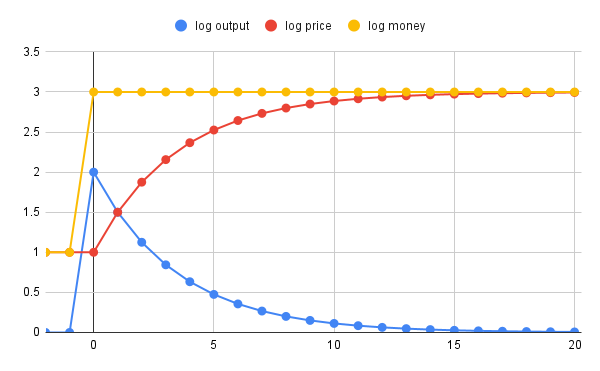
\includegraphics[width=1\textwidth]{pset4/partb.png}  % 50% of text width
        % \caption{This is an image caption.}
        \label{fig:example}
    \end{figure}

    \pagebreak
    \part

    Now suppose that $\theta = 0.5$. Trace out the dynamics in this case. 
    Again plot the results as in the previous part. 
    \\ \\
    \solution

    \begin{figure}[h]  % Optional: 'h' means "here" to place the image roughly where it appears in the code
        \centering
        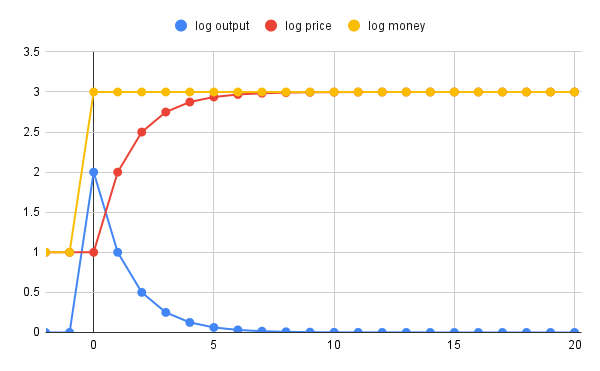
\includegraphics[width=1\textwidth]{pset4/partc.png}  % 50% of text width
        % \caption{This is an image caption.}
        \label{fig:example}
    \end{figure}

    \pagebreak
    \part

    Comment on the transiton dynamics and the difference between the two
    cases. Relate to the concept of the half-life (one paragraph). 
    \\ \\
    \solution

    Steady state logarithms of output and price are reached quicker in 
    the second case where the speed of the price adjustment, $\theta$,
    is equal to 0.5, whereas in the first case it is 0.25. The half-life
    is the time required for, in this case, the logarithms of output and
    price to reduce to half their value. In the second case, the half-life
    is then naturally shorter. This makes sense considering that, if prices
    take less time to adjust, suppliers will adjust prices quicker to
    catch up with inflated demand, thereby reducing output quicker as well. 
     

\end{homeworkProblem}

\pagebreak

\begin{homeworkProblem}[2]
    Consider again the model of the medieval economy discussed in class: 
    
    \begin{enumerate}[topsep=15pt]
        \item[] \quad \quad \:\:\: $\log M_t + \log V = \log P_t + \log Y_t$
        \item[] \quad \quad \:\:\: $\log P_{t+1} - \log P_t = \theta (\log Y_t - \log Y^*)$
    \end{enumerate}

    We would liek to rewrite the model in terms of inflation and the ``output
    gap"---i.e., the gap between actual output and steady state ouput. We denote
    inflation by $\pi_t$. Recall that inflation is defined as $\left( P_{t+1}-P_t \right)  /P_t$.
    For inflation rates close to zero the following approximation is quite accurate 
    $\pi_t \approx \log (1+\pi_t) = \log (P_t/P_{t-1})$. Please make use of this
    as needed in solving the problem. We denote the output gap by $\Tilde{Y_t}= \log Y_t - \log Y^*$.
    \\ \\
    A) Using this notation, show that the medieval economy model can be rewritten
    as:
    
    \begin{flalign*}
        & \quad \quad \text{AD:} \quad \quad \Delta \log M_t = \pi_t + \widetilde{Y_t} - \widetilde{Y}_{t-1} &\\
        & \quad \quad \text{SRAS:} \quad \pi_t = \theta \widetilde{Y}_{t-1} &\\
    \end{flalign*}

    
    where AD stands for ``aggregate demand" and SRAS stands for ``short-run 
    aggregate supply." These labels will be explained in class.
    \\ \\
    In the simplest version of the medieval economy, the money supply is
    exogenously given by, say, the number of gold coins in the economy. 
    Suppose now that the government starts issuing paper money and can thus
    change the supply of the money at will. 
    \\ \\
    For simplicity, suppose the economy is in a steady state with zero 
    inflation at time 0. In other words, $\pi_0 = 0$ and $\Tilde{Y}_0 = 0$.
    Also, assume that $\theta = 0.25$. 
    \\ \\
    B) By an unfortunate turn of events, a crazy person takes over as the 
    chairman of the central bank in our medieval economy with paper money. 
    Suppose this person decides to raise the money supply by one log unit 
    every odd period and reduce it by one log unit every even period. In
    other words $\Delta \log M_t = 1$ in odd periods and $\Delta \log M_t
    = -1$ in even periods. Solve for the dynamics of the output gap and
    inflation for 20 periods in this case.
    \\ \\
    C) The dynamics that come out of part (b) may strike you as strange. 
    Do, you think this is actually what would happen if such a crazy 
    person were to take over at the central bank? Remember that the logic
    of the model is that the reason why output deviates from desired output
    is that producers are surprised by changes in the stock of money. We 
    motivated this assumption by the notion that in the medieval economy 
    without paper money the money supply rarely changed and any changes 
    were true surprises. Remembering that the producers are trying to 
    achieve a zero output gap, explain how their behavior may eventually 
    differ from the behavior embodied in the SRAS equation above.
    \\ \\
    Now suppose that the crazy central banker is thrown out of office 
    (this is not the answer I am looking for in part C)) and the money 
    supply doesn’t change for a while so that economy again settles 
    down to the steady state with zero inflation. At that point, a new 
    central banker is hired and (s)he decides to start steadily increasing 
    the money supply. More specifically, suppose the money supply grows 
    at a constant rate $\Delta \log M_t = \Delta \log M$.
    \\ \\
    D) Assuming that the behavior of the people in the economy is well
    described by the AD and SRAS equations above, what is the steady 
    state value of the output gap and inflation for this economy as a 
    function of $\Delta \log M$?
    \\ \\
    E) Again assuming that the behavior of the people in the economy 
    is well described by the AD and SRAS equations above, plot the 
    relationship between steady state inflation and the steady state 
    output gap for different constant values of money growth with 
    inflation on the vertical axis and the output gap on the horizontal 
    axis. We refer to this relationship as the “long run aggregate supply” 
    (LRAS) relationship in the medieval model.
    \\ \\
    F) The following quote is attributed to Abraham Lincoln: “You can 
    fool some of the people all of the time, and all of the people some 
    of the time, but you cannot fool all of the people all of the time.” 
    Discuss the realism of the price setting behavior that underlies the
    SRAS curve in light of the LRAS curve derived above and Lincoln’s quote.



    \pagebreak
    \part

    Derive a production function of the form $Y=f(L)$, and derive an expression 
    for TFP of this production function. 
    \\ \\
    \solution
    \\
    A production function of the form $Y=f(L)$ given in the problem specification 
    could be the following
    \[
        \begin{split}
            Y &= (sL)^{\alpha}((1-s)L)^{1-\alpha}
            \\
            Y &= s^{\alpha}(1-s)^{1-\alpha}L
        \end{split}
    \]
    The production function is broken into two tasks, $X_1$ and $X_2$, where
    $X_1$ is the task that requires $s$ units of labor and $X_2$ is the task
    that requires $(1-s)$ units of labor. The total output $Y$ is the product
    of the output of each task.
    \\ \\
    Total Factor Productivity is the ratio of output to input, or that portion
    of growth not explained by the change in inputs. In our case, we can 
    divide output by the change in the labor input to find TFP.
    \[
        A = \frac{Y}{L} = s^{\alpha}(1-s)^{1-\alpha}
    \]
    
    \pagebreak
    \part

    Draw how TFP depends on the task allocation $s$ (recall $s \in [0,1])$.
    \\ \\
    
    \solution
    \\
    Below I have plotted three different TFP functions for different values
    of $\alpha$. The first plot is for $\alpha = 0.25$, the second plot is
    for $\alpha = 0.5$, and the third plot is for $\alpha = 0.75$. The
    general shape of the TFP function is a bell curve with a maximum at
    $s = \alpha$.
    \\
    % \begin{figure}[h!]
    %     \centering
    %     \begin{subfigure}{0.3\textwidth}
    %         \centering
    %         \begin{tikzpicture}
    %             \begin{axis}[
    %                 width=\textwidth,
    %                 height=0.8\textwidth,
    %                 xlabel={$s$},
    %                 ylabel={},
    %                 domain=0:1,
    %                 samples=100,
    %                 ymin=0, ymax=1,
    %                 axis lines=middle,
    %                 xtick={\empty},
    %                 ytick={\empty},
    %                 title={$ \alpha = 0.25 $},
    %                 xlabel style={at={(axis description cs:1,-0.1)}, anchor=north},]
    %                 \addplot[red, thick] {x^0.25*(1-x)^0.75};
    %             \end{axis}
    %         \end{tikzpicture}
    %     \end{subfigure}
    %     \begin{subfigure}{0.3\textwidth}
    %         \centering
    %         \begin{tikzpicture}
    %             \begin{axis}[
    %                 width=\textwidth,
    %                 height=0.8\textwidth,
    %                 xlabel={$s$},
    %                 domain=0:1,
    %                 samples=100,
    %                 ymin=0, ymax=1,
    %                 axis lines=middle,
    %                 xtick={\empty},
    %                 ytick={\empty},
    %                 title={$ \alpha = 0.5 $},
    %                 xlabel style={at={(axis description cs:1,-0.1)}, anchor=north},]
    %                 \addplot[red, thick] {x^0.5*(1-x)^0.5};
    %             \end{axis}
    %         \end{tikzpicture}
    %     \end{subfigure}
    %     \begin{subfigure}{0.3\textwidth}
    %         \centering
    %         \begin{tikzpicture}
    %             \begin{axis}[
    %                 width=\textwidth,
    %                 height=0.8\textwidth,
    %                 xlabel={$s$},
    %                 domain=0:1,
    %                 samples=100,
    %                 ymin=0, ymax=1,
    %                 axis lines=middle,
    %                 xtick={\empty},
    %                 ytick={\empty},
    %                 title={$ \alpha = 0.75 $},
    %                 xlabel style={at={(axis description cs:1,-0.1)}, anchor=north},]
    %                 \addplot[red, thick] {x^0.75*(1-x)^0.25};
    %             \end{axis}
    %         \end{tikzpicture}
    %     \end{subfigure}
    % \end{figure}
    \\
    From the above plots we can see that TFP is maximized at some value of $s$
    between 0 and 1. The exact value of $s$ that maximizes TFP is $\alpha$,
    which is shown in the next part.

    \pagebreak
    \part

    What is the output maximizing allocation $s^*$? What happens to TFP then?
    \\ \\
    \solution
    \\
    Output in this case is maximized when TFP is maximized. We can find the
    optimal allocation $s^*$ by taking the derivative of TFP with respect 
    to a change in $s$ and setting the result equal to zero
    \[
        \begin{split}
            \frac{dA}{ds} &= \frac{d}{ds}\left( s^\alpha(1-s)^{1-\alpha} \right)
            \\
            &= \alpha s^{\alpha-1}(1-s)^{1-\alpha} - s^{\alpha}(1-\alpha)(1-s)^{-\alpha}   
            \\
            0 &= \alpha s^{\alpha-1}(1-s)^{1-\alpha} - s^{\alpha}(1-\alpha)(1-s)^{-\alpha}   
            \\
            s^{\alpha}(\alpha-1)(1-s)^{-\alpha} &= \alpha s^{\alpha-1}(1-s)^{1-\alpha}
            \\
            s^{\alpha}(1-\alpha) &= \alpha s^{\alpha-1}(1-s)
            \\
            s(1-\alpha) &= \alpha (1-s)
            \\
            s-s\alpha &= \alpha - \alpha s
            \\
            s &= \alpha
        \end{split}
    \]

    From this we can see the optimal allocation $s^*$ is reached when 
    $s = \alpha$. At this point, TFP is maximized and the economy is
    producing output at its maximum level given a fixed amount of labor.

    \pagebreak
    \part

    In many developing countries, taxes, poor management, information problems, 
    or corruption can lead to a non-optimal allocation of tasks. How can 
    this theory explain that some countries remain poorer than the US?
    \\ \\
    \solution
    \\
    If in these developing countries there are factors that prohibit an efficient
    task allocation $s$, then TFP will be lower than it could be. Considering that
    under the Solow model there is only long run per capita growth with increasing
    TFP, these countries will remain poorer than the US and not converge to the 
    same level of output and output per capita if their allocation of labor remains
    inefficient.
    
    
        
\end{homeworkProblem}

\pagebreak
\end{document}
